\documentclass[preprint,12pt]{elsarticle}

% ── Packages ─────────────────────────────────────────────────────────────────
\usepackage[utf8]{inputenc}
\usepackage[T1]{fontenc}
\usepackage{lmodern}
\usepackage{amsmath,amssymb,amsthm}
\usepackage{mathtools}
\usepackage{bm}
\usepackage{booktabs}
\usepackage{array}
\usepackage{longtable}
\usepackage{multirow}
\usepackage{graphicx}
\usepackage{xcolor}
\usepackage[colorlinks=true,
            linkcolor=blue!60!black,
            citecolor=green!50!black,
            urlcolor=blue!70!black]{hyperref}
\usepackage{algorithm}
\usepackage{algpseudocode}
\usepackage{natbib}
\usepackage{microtype}
\usepackage{setspace}
\usepackage{enumitem}
\usepackage{lineno}
\setlength{\emergencystretch}{3em}
% Placeholder for posterior numbers to be filled from the NumPyro/NUTS refit
% on the corrected species-specific channel (mos_numpyro_fit.py).
\newcommand{\refit}[1]{\textcolor{red}{[#1]}}

% ── Theorem environments ──────────────────────────────────────────────────────
\newtheorem{theorem}{Theorem}
\newtheorem{corollary}[theorem]{Corollary}
\newtheorem{lemma}[theorem]{Lemma}
\newtheorem{proposition}[theorem]{Proposition}
\newtheorem{remark}{Remark}
\theoremstyle{definition}
\newtheorem{definition}{Definition}

% ── Custom commands ───────────────────────────────────────────────────────────
\newcommand{\E}{\mathbb{E}}
\newcommand{\Var}{\operatorname{Var}}
\newcommand{\Cov}{\operatorname{Cov}}
\newcommand{\tr}{\operatorname{tr}}
\newcommand{\diag}{\operatorname{diag}}
\newcommand{\N}{\mathcal{N}}
\newcommand{\Bern}{\operatorname{Bern}}
\newcommand{\Pois}{\operatorname{Poisson}}
\newcommand{\NB}{\operatorname{NegBin}}
\newcommand{\Bin}{\operatorname{Binomial}}
\newcommand{\Dir}{\operatorname{Dir}}
\newcommand{\bx}{\bm{x}}
\newcommand{\bz}{\bm{z}}
\newcommand{\bW}{\bm{W}}
\newcommand{\bv}{\bm{v}}
\newcommand{\bX}{\bm{X}}
\newcommand{\bbeta}{\bm{\beta}}
\newcommand{\balpha}{\bm{\alpha}}
\newcommand{\bTheta}{\bm{\Theta}}
\newcommand{\bThetaB}{\bm{\Theta}_{B}}
\newcommand{\bepsilon}{\bm{\varepsilon}}
\newcommand{\bgammapsi}{\bm{\gamma}_{\psi}}
\newcommand{\bdelta}{\bm{\delta}}
\newcommand{\bw}{\bm{w}}
\newcommand{\blambda}{\bm{\lambda}}
\newcommand{\thetaNN}{\theta_{\mathrm{NN}}}
\renewcommand{\S}{\mathcal{S}}
\newcommand{\T}{\mathcal{T}}
\newcommand{\Ni}{\mathcal{N}_i}
\newcommand{\OC}{\mathcal{O}_C}
\newcommand{\OP}{\mathcal{O}_P}

\journal{Journal of Agricultural, Biological and Environmental Statistics}

% ─────────────────────────────────────────────────────────────────────────────
\begin{document}
\linenumbers

\begin{frontmatter}

\title{Multi-Source Data Fusion and Observation-Layer Identifiability
       for Count-Valued Spatio-Temporal Abundance Models}

\author[inst1]{Xulin Pan}
\ead{xxp5066@psu.edu}
\address[inst1]{Pennsylvania State University,
  University Park, PA 16802, USA}

\author[inst2]{Jun Lv}
\address[inst2]{School of Mathematics and Statistics, Yunnan University,
  Kunming 650091, Yunnan, China}

\author[inst3]{Chuanming Wang}
\address[inst2]{School of Biological and Food Engineering, Honghe University,
  Mengzi, Yunnan, China}
  
\begin{abstract}
Ecological monitoring increasingly combines complementary data streams---standardized
counts, occupancy detections, and citizen-science checklists---that observe the same
population through different error mechanisms. We develop a self-contained framework for
fusing a count stream and a binary detection stream through a shared count-valued
spatio-temporal latent process---an agent-based transition of density-regulated
persistence, neighbourhood colonization, and long-distance arrival that is equivalently a
hierarchical spatio-temporal count state-space model---observed through a negative-binomial
count survey and a false-positive-aware Bernoulli detection survey with optional effort
exposures. We make three contributions. First, we establish well-posedness of the latent
process: the isolated-cell chain is geometrically ergodic with an explicit stationary-mean
bound, and the full grid satisfies a conditional-mean bound under bounded dispersal. Second,
we characterise observation-layer identifiability from the Fisher information---count data
identify the count-detection product and the negative-binomial dispersion, a single binary
observation cannot separate detection intensity from the false-positive rate, and temporal
abundance variation together with the count stream restore identifiability of the joint
observation-parameter vector---results that are explicitly \emph{conditional} (given known
positive latent counts) and \emph{local} (first-order, Fisher-information), not global
guarantees. Third, a simulation study with a fully specified estimator quantifies the value
of the second stream: count-only data leave the binary detection parameter unidentified,
binary-only data weakly determine abundance scale, and dual-channel fusion recovers both
detection parameters with near-nominal coverage while improving latent-field prediction.
We then fit the model to real dual-channel mosquito surveillance data from the
National Ecological Observatory Network---overnight $\mathrm{CO}_2$-trap counts
and independent daytime-trap detections of a single vector species,
\emph{Coquillettidia perturbans}---recovering a coherent latent abundance field
whose detection parameters are identified by the informative species-specific
binary channel, exactly as the theory predicts, with the absolute abundance scale
anchored by design.
The manuscript is deliberately independent of flexible-kernel and algorithm-acceleration
developments: its contribution is the data-fusion likelihood, the conditional and local
identifiability theory, and the monitoring-design interpretation.
\end{abstract}

\begin{keyword}
Multi-source data fusion \sep
Identifiability \sep
Count process \sep
Occupancy detection \sep
Geometric ergodicity \sep
Integrated data model \sep
Hierarchical Bayesian model
\end{keyword}

\end{frontmatter}

% ─────────────────────────────────────────────────────────────────────────────
\section{Introduction}
\label{sec:intro}
% ─────────────────────────────────────────────────────────────────────────────

Modern ecological monitoring rarely relies on a single observation
protocol. A breeding-bird programme may pair territory-mapping counts with
independent presence/absence visits; a mammal survey may combine transect
counts with camera-trap or acoustic detections; a plant census may join
quadrat counts with remotely sensed occupancy. These streams observe the
same underlying population but through different error mechanisms---counts
are subject to partial detection and overdispersion, while
presence/absence records are subject to imperfect and occasionally
false-positive detection. Fusing them promises sharper inference about
abundance and detectability than either stream alone
\citep{kery2016,royle2004}, but the fusion is only useful if the combined
model is identifiable: the extra data must resolve, rather than merely
relabel, the confounding between how many individuals are present and how
readily they are observed.

This confounding is the central obstacle. A count survey with conditional
mean $\rho N$ informs only the \emph{product} of detection $\rho$ and
abundance $N$; the rescaling $\rho\mapsto c\rho$, $N\mapsto N/c$ leaves the
count likelihood essentially unchanged. Replicated-count N-mixture models
\citep{royle2004} break this ridge through within-season repeat visits, and
open-population formulations \citep{dail2011} break it through the dynamics;
occupancy models break it through detection/non-detection replication. What
is far less understood is what happens when a mechanistic, movement-explicit
count ABM---in which latent abundance propagates across space through
survival, immigration, and long-distance arrival---is observed through two
heterogeneous channels at once. Does the second stream identify the
detection parameters that the first cannot, and under what conditions?

We answer this question for a count-valued spatio-temporal ABM with a
dual-channel observation layer. The latent process is the count ABM used
throughout this line of work: non-negative integer abundances evolving by
density-regulated survival, neighbourhood immigration, and long-distance
arrivals. We are deliberately agnostic about two design choices that are
the subject of other studies---the functional form of the dispersal
kernel, and the algorithm used for posterior computation---so that the
identifiability and stability results here apply to the model class rather
than to one implementation. The simulation of Section~\ref{sec:voi}
nonetheless fixes one concrete estimator, and its coverage and error figures
are specific to that choice (Section~\ref{sec:voi-methods}).

\paragraph{Contributions.}
This paper makes three contributions, all concerning the observation model
and its behaviour rather than a new estimator.
\begin{enumerate}[label=\textbf{\arabic*.},leftmargin=1.6em]
  \item \textbf{Process well-posedness.} We show that the latent count
    process is a stable generative model: the isolated-cell chain is
    geometrically ergodic with an explicit stationary-mean bound
    (Theorem~\ref{thm:ergodic}), and the full grid satisfies a
    conditional-mean bound under any bounded dispersal allocation
    (Proposition~\ref{prop:meanbound}). Fusion is therefore built on a
    process that does not explode or drift degenerately.
  \item \textbf{Observation-layer identifiability.} A Fisher-information
    analysis (Proposition~\ref{prop:ident}) establishes exactly what each
    channel identifies: the count channel identifies $(\rho,r)$ up to the
    latent scale, a single binary observation cannot separate detection
    intensity $\kappa$ from the false-positive rate $\eta$, temporal
    abundance variation with $T\ge 2$ restores their identifiability, and
    the two conditionally independent channels jointly identify the full
    observation vector $(\rho,r,\kappa,\eta)$ given known positive latent
    counts. Both statements are explicitly conditional (on known positive
    latent counts) and local (first-order, Fisher-information), and are not
    global identifiability claims.
  \item \textbf{Value of the second stream.} A simulation study
    (Section~\ref{sec:voi}) quantifies the practical payoff: count-only
    data leave $\kappa$ unidentified, binary-only data confound the
    abundance scale and forecast poorly, and dual-channel fusion recovers
    both detection parameters with near-nominal coverage and the best
    predictive accuracy. A real application
    (Section~\ref{sec:neon-mosq}) fits the same dual-channel likelihood to NEON
    mosquito surveillance data---overnight-trap counts and independent
    daytime-trap detections of \emph{Coquillettidia perturbans}---recovering the
    latent abundance field and observation parameters, whose relative
    identifiability matches the theory.
\end{enumerate}

\paragraph{Scope.}
The paper is intentionally restricted to the statistical structure of
multi-source observation. We use a fixed, bounded dispersal allocation in the
latent process so that the effect of the observation design is not confounded
with flexible kernel learning or algorithmic acceleration. Questions about
choosing highly flexible dispersal kernels or optimizing large-scale
posterior-computation algorithms are outside the present contribution. This
scope makes the paper self-contained: every theoretical and empirical result
below concerns the shared latent count process, the two observation channels,
and the monitoring-design consequences of combining them.

The remainder of the paper is organised as follows.
Section~\ref{sec:related} situates the paper within recent work on data
fusion, identifiability, and mechanistic abundance models.
Section~\ref{sec:process} specifies the latent count process and
establishes its stability. Section~\ref{sec:obs} defines the dual-channel
observation model. Section~\ref{sec:ident} develops the identifiability
theory. Section~\ref{sec:voi} reports the value-of-information simulation.
Section~\ref{sec:neon-mosq} presents a real application, fitting the model to
NEON dual-channel mosquito surveillance data, and
Section~\ref{sec:discussion} discusses implications for monitoring
design.

% ─────────────────────────────────────────────────────────────────────────────
\section{Related Work}
\label{sec:related}
% ─────────────────────────────────────────────────────────────────────────────

\paragraph{Integrated and multi-source data models.}
Combining heterogeneous observation streams to sharpen inference about
species distribution and abundance is now an established programme.
Integrated species distribution models fuse structured surveys with
opportunistic or presence-only records by having the data sets share
components of a common linear predictor \citep{isaac2020}. Most directly
related to the present work, \citet{verhoef2025} develop an integrated data
model that combines aerial survey counts with a separate detection data set
to estimate abundance under imperfect detection and temporal dependence,
using a logistic--binomial--Poisson hierarchy in which true abundance
follows a temporally autocorrelated Poisson process. We share the goal of
fusing a count stream with a detection stream to break the
abundance--detection confounding, but differ in the latent process: rather
than a phenomenological autocorrelated Poisson, the shared field here evolves
through an explicit agent-based transition---survival, neighbourhood
immigration, and long-distance arrival (Section~\ref{sec:process})---so that
the fused data inform mechanistic demographic quantities, and we treat
identifiability as a property to be proved rather than imposed by
construction.

\paragraph{Abundance, detection, and identifiability.}
The confounding between abundance and detection is the classical obstacle in
this literature. N-mixture models \citep{royle2004} identify detection from
within-season replicate counts, and open-population extensions
\citep{dail2011} identify it from the dynamics; occupancy models identify
detection from detection/non-detection replication. This identification
is, however, known to be fragile: N-mixture abundance and detection are only
weakly separated---and can be practically non-identifiable---under unmodelled
individual heterogeneity, overdispersion, or single-visit designs
\citep{link2003,knape2015,barker2018}, so identifiability must be checked for
each observation design rather than assumed. Recent work has
sharpened the identifiability question directly: \citet{doser2024} show, by
simulation, how spatial and temporal autocorrelation can substitute for
replication in single-visit multi-season occupancy models, and
\citet{doser2023} give joint species distribution models with imperfect
detection for high-dimensional spatial data, resolving latent-factor
identifiability by construction. These treatments concern occupancy or
regression-based abundance models and establish identifiability empirically
or through modelling constraints. Our Proposition~\ref{prop:ident} instead
gives an analytical, Fisher-information characterisation for the
\emph{dual-channel} count-plus-detection layer: the count channel identifies
$(\rho,r)$ up to the latent scale, a single binary observation is
rank-deficient in $(\kappa,\eta)$, temporal abundance variation restores
identifiability, and conditional independence renders the joint information
block-diagonal. To our knowledge an observation-layer identifiability
theorem for fused count and false-positive-aware detection channels over a
mechanistic count process has not previously appeared.

\paragraph{Statistical agent-based models and dispersal.}
Mechanistic, movement-explicit models of abundance descend from the
hierarchical statistical framework of \citet{hooten2010}, who modelled
binary occupancy dynamics on a lattice with neighbourhood dispersal and
Gibbs sampling. Dispersal in such models is often encoded by fixed,
isotropic or distance-decay kernels \citep{nathan2012}. The present paper
uses a deliberately simple bounded dispersal allocation because the object of
study is not kernel learning but the observation design: how two imperfect
streams identify abundance and detection when they are linked through the
same mechanistic count process. This separation is important for statistical
clarity. If the fused observation layer is not identifiable under a fixed
kernel, adding a more flexible movement model will not solve the fundamental
abundance--detection confounding.

\paragraph{Estimator-independent theory, one estimator for the simulation.}
The identifiability and stability results below are properties of the model's
likelihood and Fisher information, and therefore do not depend on how the
likelihood is fit: they hold whether it is explored by MCMC, particle methods,
variational or Laplace approximations, or other state-space tools, provided the
same latent process and observation layer are used. The \emph{empirical}
parameter recovery, interval coverage, and predictive scores reported in
Section~\ref{sec:voi} are, by contrast, necessarily estimator-specific: a
coverage number cannot be produced without committing to an estimator, priors,
and an interval rule. We therefore fix one concrete estimator and its priors in
Section~\ref{sec:voi-methods}, and the coverage figures should be read as
properties of that estimator applied to this model, not as claims about the
model class under every possible fitting algorithm. This division---
estimator-independent theory, one fully specified estimator for the
simulation---is appropriate for JABES-style methodology: the paper contributes
the identifiable integrated-data model and its monitoring implications, not a
new optimization routine.

% ─────────────────────────────────────────────────────────────────────────────
\section{The Count-Valued Latent Process}
\label{sec:process}
% ─────────────────────────────────────────────────────────────────────────────

Let $\S=\{1,\ldots,m\}$ index spatial cells on a lattice or graph and
$t=1,\ldots,T$ index discrete time. The latent abundance
$N_{i,t}\in\mathbb{Z}_{\ge0}$ at cell $i$ and time $t$ evolves as the sum of
three conditionally independent components,
\begin{equation}
  N_{i,t}=S_{i,t}+I_{i,t}+L_{i,t},
  \label{eq:decomp}
\end{equation}
where, given the previous field $\{N_{j,t-1}\}_{j\in\S}$,
\begin{align}
  S_{i,t}
  &\sim\Bin\!\left(N_{i,t-1},\;
    \phi_i\exp(-N_{i,t-1}/K_i)\right),
  \label{eq:survival}\\
  I_{i,t}
  &\sim\Pois(\Lambda_{i,t}),\qquad
  \Lambda_{i,t}=\sum_{j:\,i\in\mathcal{N}_j}
    p_{j\to i}\,g(N_{j,t-1};\nu)\,N_{j,t-1},
  \label{eq:immigration}\\
  L_{i,t}
  &\sim\Pois(\psi_i).
  \label{eq:ldd}
\end{align}
Here $\phi_i\in(0,1)$ is a baseline persistence probability, $K_i>0$ a
carrying capacity that induces density-regulated survival, $p_{j\to i}\ge0$
the outgoing dispersal weight from source $j$ to target $i$ over the
neighbourhood $\mathcal{N}_j$, and $\psi_i>0$ a long-distance arrival rate.

Equations~\eqref{eq:decomp}--\eqref{eq:ldd} admit two equivalent readings.
Mechanistically they describe an \emph{agent-based} generative process: each of
the $N_{i,t-1}$ individuals in a cell independently survives with a
density-dependent probability, seeds recruits into neighbouring cells, and is
supplemented by arrivals, so the one-step update is the aggregate of
individual-level survival, dispersal, and arrival events. Statistically the same
equations define a hierarchical spatio-temporal count state-space model with a
Markov latent field. We retain the agent-based terminology to emphasise the
individual-level, mechanistic origin of the transition kernel, but every result
below is a statement about this state-space model and requires no agent-level
simulation.

The density-scaling function
\begin{equation}
  g(N;\nu)=\frac{N}{N+\nu},\qquad
  g(0;\nu)=0,\quad g(N;\nu)\to1\ \text{as}\ N\to\infty,
  \label{eq:density-scale}
\end{equation}
saturates the per-source contribution in the source population, with a half-saturation constant $\nu>0$ (distinct from the false-positive rate $\eta$ of the binary detection channel in Section~\ref{sec:obs}). The
dispersal weights $p_{j\to i}$ are taken here as a fixed, normalised
allocation satisfying $\sum_{i\in\mathcal{N}_j}p_{j\to i}\le1$ (each source
distributes at most a unit dispersal budget, with the residual retained
locally). The results below require only this budget constraint; they do not
require a learned or otherwise highly parameterized movement kernel.

\subsection{Conditional Moments}
\label{sec:moments}

Writing $p_{s,i,t-1}=\phi_i\exp(-N_{i,t-1}/K_i)$ for the realised survival
probability, conditional independence of $S_{i,t}$, $I_{i,t}$, $L_{i,t}$
gives
\begin{align}
  \E[N_{i,t}\mid\mathbf{N}_{t-1}]
  &=N_{i,t-1}p_{s,i,t-1}+\Lambda_{i,t}+\psi_i,
  \label{eq:cond-mean}\\
  \Var[N_{i,t}\mid\mathbf{N}_{t-1}]
  &=N_{i,t-1}p_{s,i,t-1}(1-p_{s,i,t-1})+\Lambda_{i,t}+\psi_i.
  \label{eq:cond-var}
\end{align}
Subtracting~\eqref{eq:cond-mean} from~\eqref{eq:cond-var},
\begin{equation}
  \Var[N_{i,t}\mid\mathbf{N}_{t-1}]-\E[N_{i,t}\mid\mathbf{N}_{t-1}]
  =-N_{i,t-1}p_{s,i,t-1}^{\,2}\le0,
  \label{eq:var-minus-mean}
\end{equation}
so the one-step latent transition is (weakly) underdispersed: the Binomial
survival term makes the conditional variance no larger than the conditional
mean, while the two Poisson components contribute equally to both. Any
overdispersion in observed counts must therefore be accommodated by the
observation model (Section~\ref{sec:obs}), not attributed to the latent
transition. The probability generating function of~\eqref{eq:decomp}
factorises as the product of the Binomial and two Poisson generating
functions, which is convenient for the moment computations used below.

\subsection{Stochastic Stability}
\label{sec:stability}

Fusion of observation streams is meaningful only if the shared latent
process is itself stable. We give two results: geometric ergodicity of the
isolated-cell chain, and a conditional-mean bound on the full grid.

\begin{theorem}[Geometric ergodicity of the single-cell chain]
\label{thm:ergodic}
Consider a single isolated cell ($\mathcal{N}_i=\varnothing$) with dynamics
\[
  N_t=S_t+L_t,\quad
  S_t\mid N_{t-1}\sim\Bin\!\left(N_{t-1},\phi e^{-N_{t-1}/K}\right),
  \quad L_t\sim\Pois(\psi),
\]
with $\phi\in(0,1)$, $K>0$, and $\psi>0$. Then $\{N_t\}_{t\ge0}$ is a
geometrically ergodic Markov chain on $\mathbb{Z}_{\ge0}$ with a unique
stationary distribution $\pi_\phi$ satisfying
\[
  \E_{\pi_\phi}[N]\le \frac{\phi K}{e}+\psi .
\]
\end{theorem}

\begin{proof}
\emph{Irreducibility and aperiodicity.} Because $\psi>0$, the $\Pois(\psi)$
arrivals give $\Pr(N_t=k\mid N_{t-1}=n)\ge\Pr(S_t=0)\,\Pr(L_t=k)>0$ for all
$n,k\ge0$, so the chain is $\psi$-irreducible and aperiodic on
$\mathbb{Z}_{\ge0}$ and every finite set is petite.

\emph{Geometric drift.} Take the norm-like Lyapunov function $V(n)=1+n$.
Using $e^{-n/K}\le1$ for all $n\ge0$,
\[
  \E[V(N_t)\mid N_{t-1}=n]
  =1+n\phi e^{-n/K}+\psi
  \;\le\; \phi(1+n)+(1+\psi-\phi)
  \;=\;\lambda V(n)+b,
\]
with contraction rate $\lambda=\phi\in(0,1)$ and $b=1+\psi-\phi<\infty$,
\emph{for every} $n\ge0$. This is the geometric Foster--Lyapunov drift
condition~(V4) of \citet[Ch.~15]{meyntweedie2009}, and not merely a uniform
bound on the conditional mean. The drift moreover strengthens as
$n\to\infty$: since $\phi e^{-n/K}\to0$, outside the finite set
$C_\varepsilon=\{n:\phi e^{-n/K}>\varepsilon\}$ the same inequality holds with
any rate $\varepsilon\in(0,\phi]$, so contraction is arbitrarily strong for
large $n$. With $V$ norm-like, $C_\varepsilon$ petite, and the chain
irreducible and aperiodic, \citet[Thm.~15.0.1]{meyntweedie2009} yields
geometric ergodicity and a unique stationary law $\pi_\phi$.

\emph{Mean bound.} Taking expectations under stationarity in
$\E_{\pi_\phi}[N]=\E_{\pi_\phi}\!\left[N\phi e^{-N/K}\right]+\psi$ and using
$n e^{-n/K}\le K/e$ for all $n\ge0$ (maximum at $n=K$) gives
$\E_{\pi_\phi}[N]\le \phi K/e+\psi$.
\end{proof}

\begin{remark}[The $\psi=0$ boundary]
When $\psi=0$ the chain is absorbed at $0$: once $N_t=0$, the Binomial
survival term produces no offspring and $\Pois(0)=\delta_0$ adds none, so
$0$ is absorbing and Theorem~\ref{thm:ergodic} does not apply. A strictly
positive long-distance arrival rate, $\psi_i\ge\varepsilon_0>0$, is
therefore both an ecological modelling choice (open populations receive
occasional immigrants) and a technical requirement for a non-degenerate
stationary law.
\end{remark}

\begin{proposition}[Conditional-mean bound under bounded dispersal]
\label{prop:meanbound}
On the full $m$-cell grid, let $\phi_{\max}=\max_i\phi_i<1$ and
$\Psi=\sum_i\psi_i$. For any dispersal allocation satisfying
$\sum_{i\in\mathcal{N}_j}p_{j\to i}\le1$,
\[
  \E\!\left[\sum_{i=1}^m N_{i,t}\;\Big|\;\mathbf{N}_{t-1}\right]
  \;\le\;
  \phi_{\max}\sum_{i=1}^m N_{i,t-1}
  \;+\;\sum_{j=1}^m g(N_{j,t-1};\nu)\,N_{j,t-1}\cdot\!\!
       \sum_{i\in\mathcal{N}_j}p_{j\to i}
  \;+\;\Psi ,
\]
and since $\sum_{i\in\mathcal{N}_j}p_{j\to i}\le1$ and $g\le1$ the
immigration term is bounded by $\sum_j N_{j,t-1}$. The self-retention
allocation satisfies the strict inequality
$\sum_{i\in\mathcal{N}_j}p_{j\to i}<1$, so total abundance does not grow
without bound whenever survival and re-dispersal together remain
sub-conservative.
\end{proposition}

\begin{proof}[Proof sketch]
Sum~\eqref{eq:cond-mean} over $i$, bound each survival term by
$\phi_{\max}N_{i,t-1}$ using $e^{-N/K}\le1$, and regroup the immigration
double sum by source $j$, using
$\sum_{i\in\mathcal{N}_j}p_{j\to i}\le1$ and $g\le1$.
\end{proof}

Together, Theorem~\ref{thm:ergodic} and Proposition~\ref{prop:meanbound}
establish that the latent field to be observed is a stable, non-explosive
process with a well-defined equilibrium scale---the setting in which asking
what the observations identify is meaningful. We emphasise that
Proposition~\ref{prop:meanbound} bounds the conditional mean of the total,
not a global stability theorem for every cell; the neighbourhood term is a
local recruitment or colonization pressure rather than a mass-conserving
relocation.

\subsection{Numerical validation of the process}
\label{sec:sim-validation}

We verify the generative model and its analytical properties by direct
simulation of the count ABM on a $15\times15$ lattice over $T=60$ time steps,
with heterogeneous, covariate-driven demographic parameters and the
softmax-with-retention dispersal allocation (whose realised budget
$\max_j\sum_{i}p_{j\to i}\approx 0.91<1$ satisfies the constraint of
Proposition~\ref{prop:meanbound}). The simulation and the Monte-Carlo checks
below are produced by the reference implementation released with the paper
(\texttt{sc\_abm\_model.py}).

Figure~\ref{fig:sim} summarises one realisation. Total latent abundance rises
from its seeded value and settles onto a fluctuating plateau (panel~a),
consistent with the non-explosive behaviour guaranteed by
Proposition~\ref{prop:meanbound}; individual cells equilibrate at levels set
by their heterogeneous carrying capacities $K_i$ (panels~b--c), and the latent
field at the final time (panel~d) shows the spatial structure induced by
habitat-driven $K_i$ and neighbourhood dispersal. Panels~(e)--(f) display the
two observation channels formalised in Section~\ref{sec:obs}: negative-binomial
counts with missing cells, and the Bernoulli detection probability
$\pi_{i,t}=\eta+(1-\eta)(1-e^{-\kappa N_{i,t}})$.

Figure~\ref{fig:diag} validates the two process results that underpin the
fusion analysis. The left panel confirms the one-step underdispersion
identity~\eqref{eq:var-minus-mean},
$\Var[N_{i,t}\mid\mathbf{N}_{t-1}]-\E[N_{i,t}\mid\mathbf{N}_{t-1}]
=-N_{i,t-1}p_{s}^{2}\le0$: Monte-Carlo estimates (points) track the closed form
(curve) across the range of previous-state abundances, and the difference is
non-positive throughout---so any observed overdispersion is attributable to the
observation model rather than to the latent transition. The right panel shows
the empirical stationary law of the isolated-cell chain
(Theorem~\ref{thm:ergodic}): the chain concentrates on a stable distribution
whose mean ($\approx 2.9$ in this configuration) lies well within the
analytical bound $\phi K/e+\psi\approx 13.9$, numerically confirming geometric
ergodicity and the stationary-mean bound.

\begin{figure}[t]
\centering
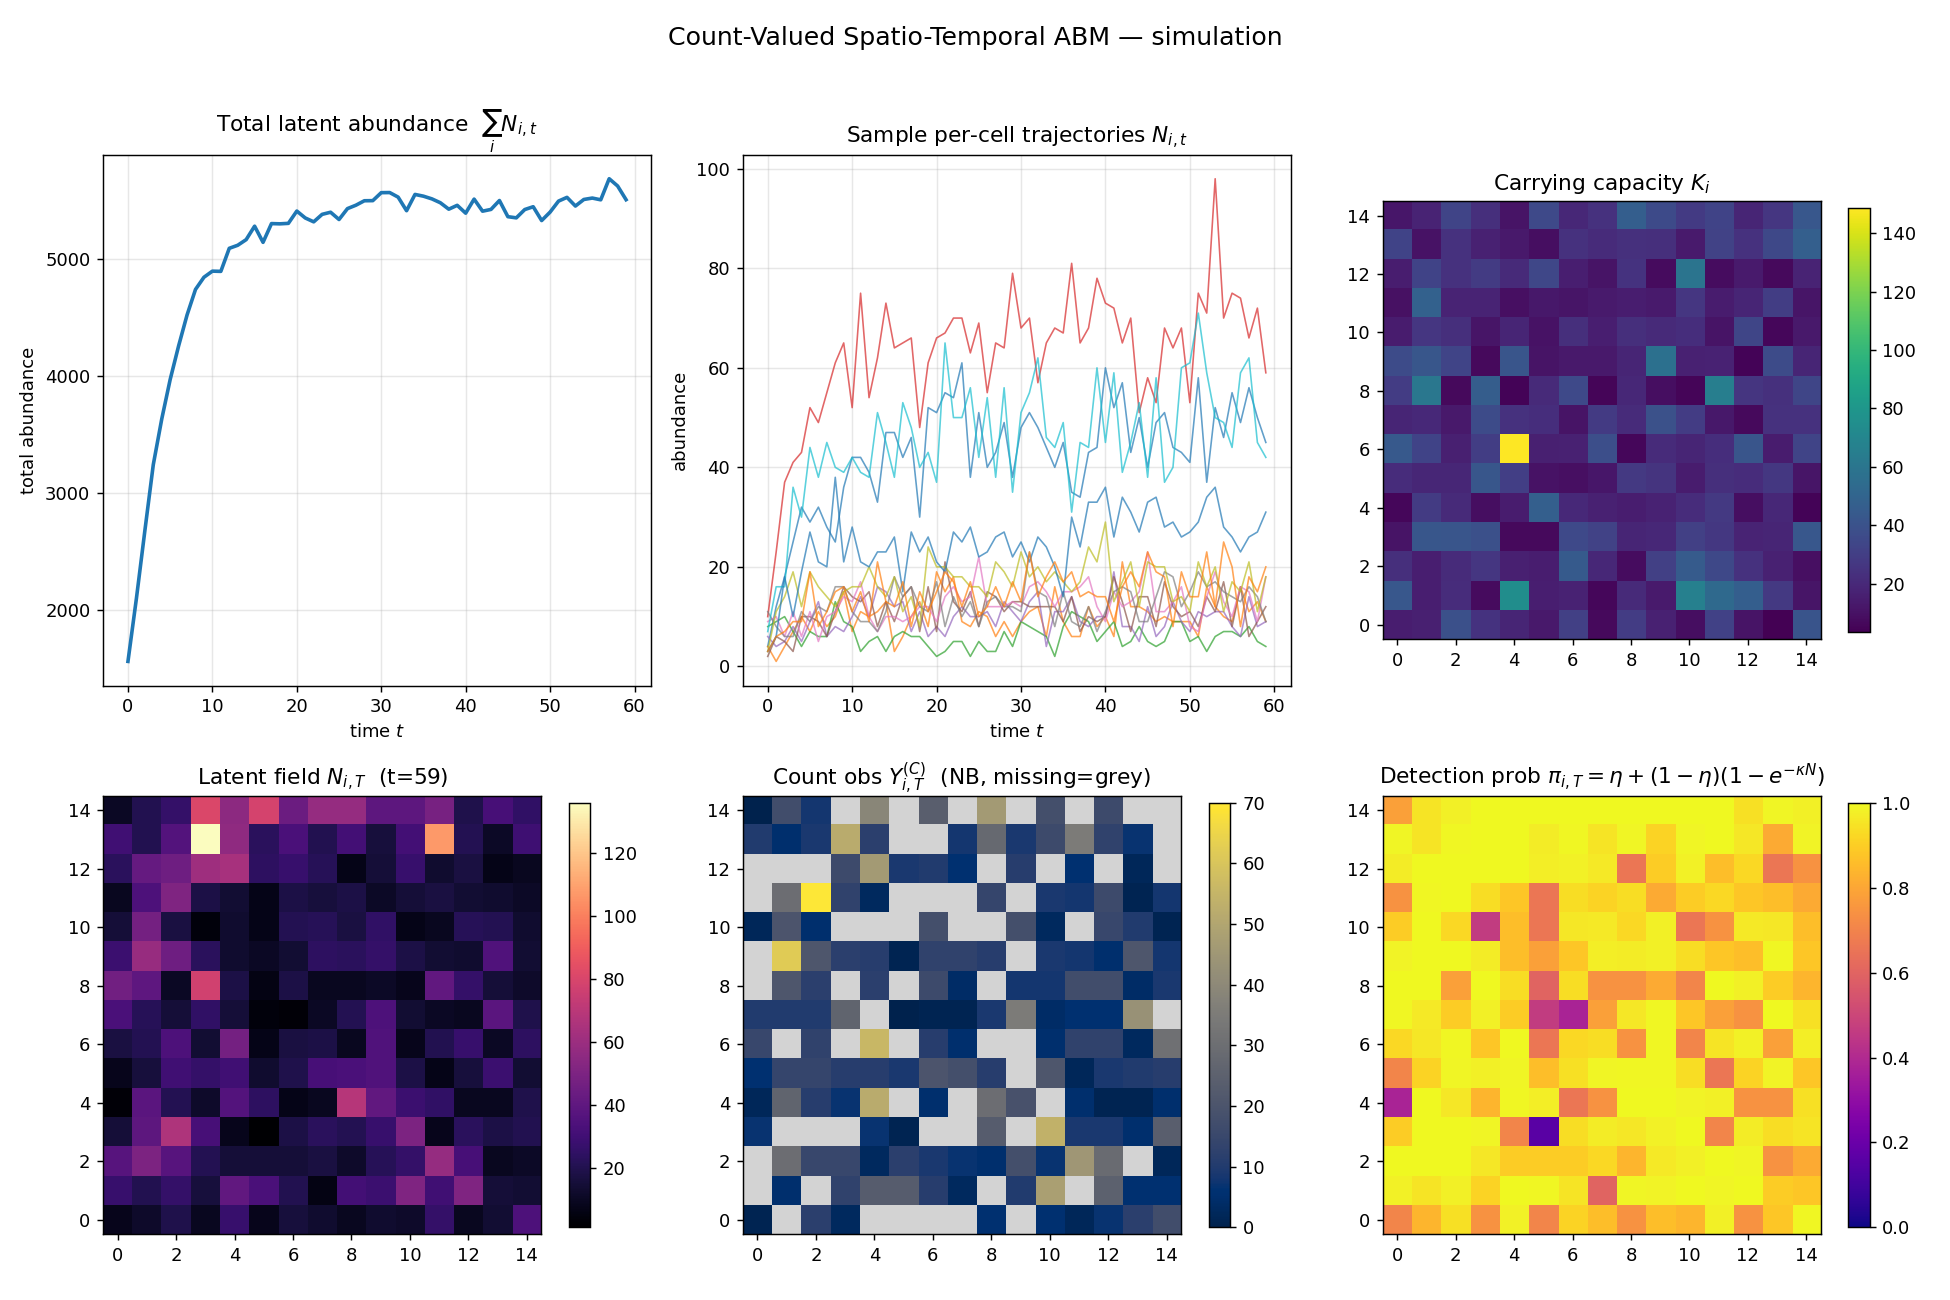
\includegraphics[width=\textwidth]{sc_abm_simulation.png}
\caption{Simulation of the count ABM on a $15\times15$ lattice ($T=60$).
(a)~total latent abundance $\sum_i N_{i,t}$ reaching a stable plateau;
(b)~sample per-cell trajectories $N_{i,t}$; (c)~heterogeneous carrying
capacities $K_i$; (d)~latent field $N_{i,T}$ at the final time;
(e)~negative-binomial count observations $Y^{(C)}_{i,T}$ (grey${}={}$missing);
(f)~binary-channel detection probability
$\pi_{i,T}=\eta+(1-\eta)(1-e^{-\kappa N_{i,T}})$.
Panels~(e)--(f) illustrate the two observation channels of
Section~\ref{sec:obs}.}
\label{fig:sim}
\end{figure}

\begin{figure}[t]
\centering
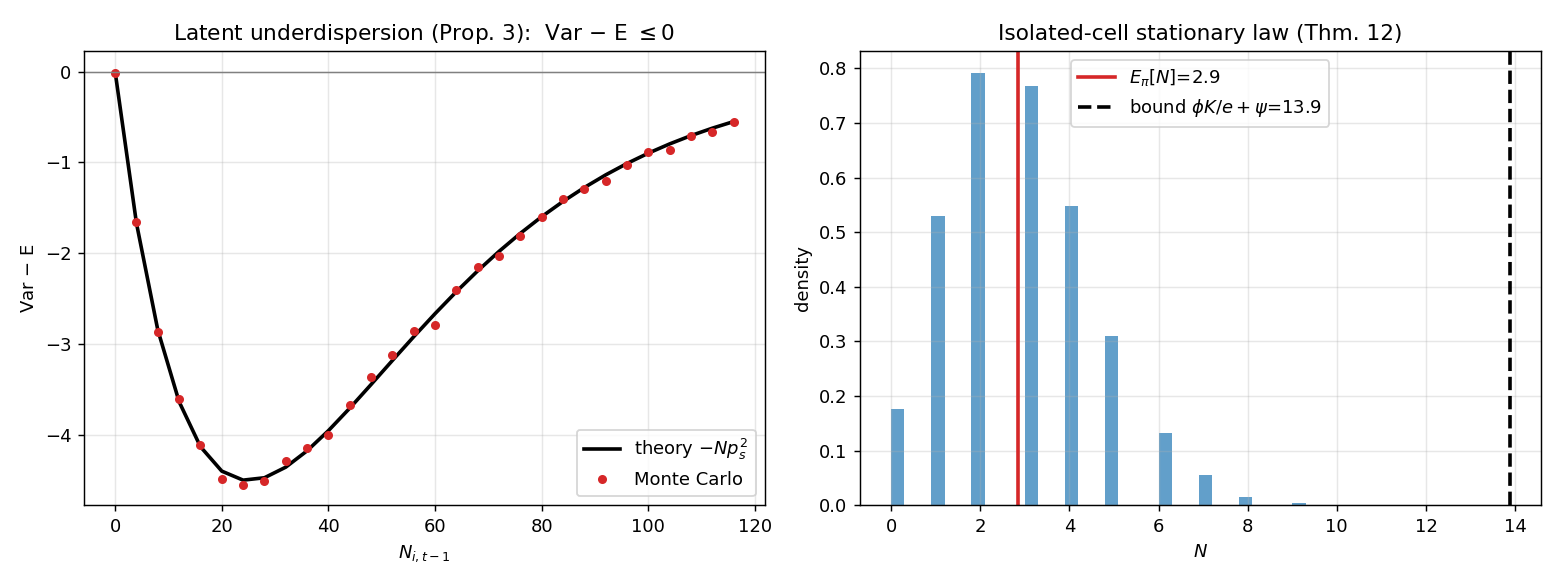
\includegraphics[width=\textwidth]{sc_abm_diagnostics.png}
\caption{Monte-Carlo validation of the process properties.
\emph{Left:} the one-step underdispersion identity~\eqref{eq:var-minus-mean},
$\Var-\E=-N_{i,t-1}p_{s}^{2}\le0$: simulated moments (points) match the closed
form (solid curve). \emph{Right:} the empirical stationary distribution of the
isolated-cell chain (Theorem~\ref{thm:ergodic}); its mean (solid line) lies
well within the analytical bound $\phi K/e+\psi$ (dashed line), numerically
confirming geometric ergodicity. The left panel aggregates $120{,}000$
Monte-Carlo draws at each of $30$ previous-state values $N_{i,t-1}$; the right
panel uses a single isolated-cell chain of $40{,}000$ steps with the first
$2{,}000$ discarded as burn-in ($38{,}000$ retained draws).}
\label{fig:diag}
\end{figure}

% ─────────────────────────────────────────────────────────────────────────────
\section{The Dual-Channel Observation Model}
\label{sec:obs}
% ─────────────────────────────────────────────────────────────────────────────

The observation layer is the object of this paper. Let
$\OC\subseteq\S\times\{1,\ldots,T\}$ index observed count-survey cell--time
pairs and $\OP\subseteq\S\times\{1,\ldots,T\}$ index observed binary
detection pairs. The central modelling assumption is that both channels are
conditionally independent given the shared latent field $\{N_{i,t}\}$.

\subsection{Count Survey Channel}

For $(i,t)\in\OC$,
\begin{equation}
  \begin{aligned}
  Y^{(C)}_{i,t}\mid N_{i,t},\rho_{i,t},r
  &\sim\NB(\rho_{i,t}N_{i,t},\,r),\\
  \Var[Y^{(C)}_{i,t}\mid N_{i,t}]
  &=\rho_{i,t}N_{i,t}\!\left(1+\frac{\rho_{i,t}N_{i,t}}{r}\right),
  \end{aligned}
  \label{eq:count-channel}
\end{equation}
with detection fraction $\rho_{i,t}\in(0,1)$ and overdispersion parameter
$r>0$; $r\to\infty$ recovers the Poisson. The negative-binomial form
absorbs survey overdispersion and zero-inflation relative to a Poisson
observation model \citep{royle2004,kery2016}. When effort covariates
$\bm{e}_{i,t}$ are available one may model
$\operatorname{logit}(\rho_{i,t})=\mu_\rho+\bdelta^\top\bm{e}_{i,t}+v_i$;
in what follows we treat $\rho_{i,t}\equiv\rho$ and $r$ as constants for the
identifiability analysis.

\subsection{Binary Detection Channel}

For $(i,t)\in\OP$,
\begin{equation}
  Y^{(P)}_{i,t}\mid N_{i,t},\kappa,\eta
  \sim\Bern(\pi_{i,t}),\qquad
  \pi_{i,t}=\eta+(1-\eta)\bigl(1-e^{-\kappa N_{i,t}}\bigr),
  \label{eq:binary-channel}
\end{equation}
where $\kappa>0$ is the per-individual detection intensity and
$\eta\in[0,1)$ is a false-positive probability. The term
$1-e^{-\kappa N_{i,t}}$ is the probability that at least one of $N_{i,t}$
individuals, each generating a detectable signal at rate $\kappa$, is
recorded; the false-positive term $\eta$ allows a detection even when the
site is unoccupied. Key properties:
\begin{equation}
  N_{i,t}=0\ \Rightarrow\ \Pr(Y^{(P)}_{i,t}=1)=\eta,
  \qquad
  N_{i,t}\to\infty\ \Rightarrow\ \Pr(Y^{(P)}_{i,t}=1)\to1 .
  \label{eq:binary-props}
\end{equation}
Setting $\eta=0$ recovers a no-false-positive detection channel; the
special case $\pi_{i,t}=1-e^{-\kappa N_{i,t}}$ with $\eta=0$ reduces to the
saturating occupancy data model of \citet{hooten2010}. Habitat products
such as forest or tree cover are \emph{not} direct detections of the focal
species and should enter as environmental covariates on $K_i$ and $\phi_i$
rather than as $Y^{(P)}$, unless an explicit false-positive proxy is
specified.

\subsection{Joint Observation Likelihood}

Conditional independence given $\mathbf{N}$ gives
\begin{equation}
\begin{aligned}
  \mathcal{L}\!\left(\mathbf{Y}^{(C)},\mathbf{Y}^{(P)}
    \mid\mathbf{N},\rho,r,\kappa,\eta\right)
  ={}&\prod_{(i,t)\in\OC}
    \NB\!\left(Y^{(C)}_{i,t};\rho N_{i,t},r\right)\\
  &{}\times\prod_{(i,t)\in\OP}
    \Bern\!\left(Y^{(P)}_{i,t};
      \eta+(1-\eta)(1-e^{-\kappa N_{i,t}})\right).
\end{aligned}
  \label{eq:joint-likelihood}
\end{equation}
The count channel supplies abundance-scale information through
$\E[Y^{(C)}_{i,t}]=\rho N_{i,t}$, while the binary channel supplies
complementary evidence about presence through $\kappa N_{i,t}$. Whether the
two together resolve the abundance--detection confounding is the subject of
the next section.

\begin{remark}[Intuition for dual-channel identification]
\label{rmk:intuition}
Condition on a known positive latent count $N_{i,t}>0$. The count channel
constrains $\rho$ through $\E[Y^{(C)}_{i,t}]=\rho N_{i,t}$; with $N$ and
$\rho$ fixed, the binary probability
$\pi=\eta+(1-\eta)(1-e^{-\kappa N})$ is strictly increasing in $\kappa$ for
$N>0$ and $\eta<1$, and so identifies $\kappa$ by inversion---provided
$\eta$ is known or pinned by replication. The requirement in both cases is
$N_{i,t}>0$ and temporal variation in $N$; without abundance variation
$\kappa$ and $\eta$ remain confounded, as made precise below.
\end{remark}

% ─────────────────────────────────────────────────────────────────────────────
\section{Identifiability of the Observation Layer}
\label{sec:ident}
% ─────────────────────────────────────────────────────────────────────────────

We now characterise, through the Fisher information, exactly what each
channel identifies. Throughout, ``conditional observation-layer
identifiability'' means local identifiability of the observation parameters
given the latent counts $\{n_{i,t}\}$ treated as known and positive; the
implications for the fully latent case are discussed afterwards.

\begin{proposition}[Dual-channel local identifiability]
\label{prop:ident}
Consider the observation model at a single cell $i$ with known latent
counts $n_{i,1},\ldots,n_{i,T}>0$ and parameters $(\rho,r,\kappa,\eta)$.
\begin{enumerate}[label=\emph{(\roman*)},leftmargin=2.2em]
  \item \textbf{Count channel.} The negative-binomial log-likelihood has
    Fisher information
    \[
      I_{\rho\rho}=\frac{nr}{\rho(r+\rho n)}>0,
      \qquad
      I_{rr}=\sum_{k\ge0}\bigl[s_r(k)\bigr]^2\,\NB(k;\rho n,r)>0,
    \]
    where
    $s_r(k)=\partial_r\log\NB(k;\rho n,r)
      =\psi^{(0)}(r+k)-\psi^{(0)}(r)+\log\frac{r}{r+\rho n}+\frac{\rho n-k}{r+\rho n}$
    is the dispersion score and $\psi^{(0)}$ the digamma function. By the
    information identity this equals
    $I_{rr}=\sum_{k\ge0}\bigl[\psi^{(1)}(r)-\psi^{(1)}(r+k)\bigr]\NB(k;\rho n,r)
      -\rho n/\{r(r+\rho n)\}$, with $\psi^{(1)}$ the trigamma function, and
    is strictly positive because the dispersion score is not almost surely
    zero for any $r>0$. Hence $(\rho,r)$ are jointly locally identifiable from the
    count channel alone provided
    $n>0$; the dispersion $r$ is separately identified through the variance
    inflation $\Var(Y^{(C)})/\E[Y^{(C)}]=1+\rho n/r>1$.
  \item \textbf{Binary channel at fixed abundance.} With
    $\pi=\eta+(1-\eta)(1-e^{-\kappa n})$, the Bernoulli information for
    $(\kappa,\eta)$ is
    \[
      I^{(P)}_{\kappa,\eta}(n)
      =\frac{e^{-2\kappa n}}{\pi(1-\pi)}
      \begin{pmatrix}
        (1-\eta)^2 n^2 & (1-\eta)n\\[2pt]
        (1-\eta)n & 1
      \end{pmatrix}.
    \]
    This matrix has rank $1$: at a single fixed abundance $n$, $\kappa$ and
    $\eta$ are \emph{not} separately identifiable.
  \item \textbf{Binary channel with temporal variation.} If $T\ge2$ and
    $n_{i,1}\ne n_{i,2}$, the accumulated information
    $\sum_{t}I^{(P)}_{\kappa,\eta}(n_{i,t})$ is positive definite, with
    \[
      \det\!\Bigl(\sum_t I^{(P)}_{\kappa,\eta}(n_{i,t})\Bigr)
      =\frac{(1-\eta)^2 e^{-2\kappa(n_{i,1}+n_{i,2})}(n_{i,1}-n_{i,2})^2}
             {\pi_{i,1}(1-\pi_{i,1})\,\pi_{i,2}(1-\pi_{i,2})}>0 .
    \]
    Under the process model $n_{i,t}$ varies whenever $\psi_i>0$ or the
    dispersal network is non-trivial, so $(\kappa,\eta)$ are locally
    identifiable from the binary channel with $T\ge2$.
  \item \textbf{Dual-channel identifiability.} Because the two channels are
    conditionally independent given $\mathbf{N}$, the joint Fisher
    information is block-diagonal in $(\rho,r)$ and $(\kappa,\eta)$. Under
    \emph{(i)} and \emph{(iii)}, the full observation vector
    $(\rho,r,\kappa,\eta)$ is locally identifiable given known positive
    latent counts, for $T\ge2$, $\kappa>0$, $0<\eta<1$.
\end{enumerate}
\end{proposition}

\begin{proof}[Proof sketch]
Parts \emph{(i)}--\emph{(ii)} are direct computations of the log-likelihood
Hessians of~\eqref{eq:count-channel} and~\eqref{eq:binary-channel} in
expectation. The rank-one structure in \emph{(ii)} follows because both
entries of the score are proportional to the single quantity
$\partial\pi/\partial(\kappa,\eta)$ evaluated at a fixed $n$. Part
\emph{(iii)} sums two rank-one matrices at distinct abundances, whose
determinant is the stated Cauchy--Schwarz gap, positive iff
$n_{i,1}\ne n_{i,2}$. Part \emph{(iv)} is block-diagonality of the joint
information under conditional independence, so positive definiteness of each
block gives positive definiteness of the whole.
\end{proof}

\begin{remark}[Why the second stream is necessary, not merely convenient]
\label{rmk:necessary}
Proposition~\ref{prop:ident} makes the confounding precise. With only count
data ($\OP=\varnothing$), the false-positive rate $\eta$ and the detection
intensity $\kappa$ are unidentified because the binary channel is absent
entirely; with only binary data ($\OC=\varnothing$), the count dispersion
$r$ and detection fraction $\rho$ are confounded with the latent scale. A
\emph{single} time point of binary data cannot separate $\kappa$ from
$\eta$ (part \emph{(ii)}), so temporal replication is not optional for
binary-channel calibration. The dual-channel design is therefore necessary,
not merely convenient, for recovering the full observation-parameter
vector.
\end{remark}

\begin{remark}[Conditional versus hierarchical identifiability]
\label{rmk:conditional}
Proposition~\ref{prop:ident} conditions on the latent field
$\{n_{i,t}\}$ being known and positive. Because abundance is in fact latent,
full hierarchical identifiability additionally requires that the marginal
distribution of the observations determine the parameters given the process
law---a stronger property that depends on the process parameters and cannot
be read off the observation layer alone. When $\eta$ is left free, a further
degeneracy arises: at any single time point, increasing $\eta$ and
decreasing $\kappa$ can match the same detection probability. Sufficient
remedies include (a)~spatial replication with a shared $\eta$ across cells,
(b)~temporal replication with time-constant $\eta_i$ and $T\ge3$, or (c)~an
informative prior concentrating $\eta$ near zero (e.g.\
$\eta\sim\mathrm{Beta}(1,20)$ for a clean instrument). We recommend (c) with
a sensitivity analysis, and treat the conditional result as a necessary
structural condition whose practical bite is assessed empirically in
Section~\ref{sec:voi}.
\end{remark}

% ─────────────────────────────────────────────────────────────────────────────
\section{The Value of the Second Stream: Simulation}
\label{sec:voi}
% ─────────────────────────────────────────────────────────────────────────────

The identifiability theory conditions on known latent counts; the
practically relevant question is whether the detection parameters are
recoverable when abundance is unobserved. We answer it by simulation.
Independent replicates are generated from the count ABM of
Section~\ref{sec:process} at known parameters ($m=100$, $T=20$, $R=100$),
with true binary detection intensity $\kappa^\star=0.08$ and true detection
intercept $\mu_\rho^\star=-1.0$, and fitted under three observation
regimes:
\begin{itemize}[leftmargin=1.5em]
  \item \textbf{R1 (count only):} $\OP=\varnothing$; only the
    negative-binomial counts are observed.
  \item \textbf{R2 (binary only):} $\OC=\varnothing$; only the Bernoulli
    detections are observed.
  \item \textbf{R3 (multi-source):} both channels observed, sharing the
    latent field.
\end{itemize}
Predictive metrics are computed on a common held-out count-and-binary test
set of the final time steps. We report the root-mean-square error and
$95\%$ interval coverage for $\kappa$ and $\mu_\rho$, the latent-field mean
squared prediction error ($N$ MSPE), the predictive log-likelihood (PLL),
and the energy score (ES; \citealp{gneiting2007}, which coincides with the
CRPS for univariate predictions).

\subsection{Estimation and evaluation}
\label{sec:voi-methods}

\paragraph{Estimator.}
The identifiability and stability results of
Sections~\ref{sec:process}--\ref{sec:ident} are properties of the likelihood
and hold however it is fit, but the recovery and coverage numbers in
Table~\ref{tab:voi} are produced by a specific estimator, which we now fix.
Within each replicate the latent count field $N_{1:T}$ is integrated out
\emph{exactly} by a truncated forward (hidden-Markov) filter on the integer
state space $\{0,1,\dots,N_{\max}\}$ with $N_{\max}=200$, the truncated tail
mass being placed on the top state. This yields the exact log marginal
likelihood $\ell(\theta_{\mathrm{obs}})$ of the observation-parameter vector
$\theta_{\mathrm{obs}}=(\mu_\rho,r,\kappa,\eta)$ up to state truncation, with
the process parameters $(\phi,\psi)$ and the carrying-capacity scale held at
their data-generating values---the conditional regime isolated by
Proposition~\ref{prop:ident}. Holding the process fixed isolates the observation
layer but understates uncertainty; Appendix~\ref{app:robust} repeats the analysis
with $(\phi,\psi,K)$ estimated jointly and in a low-abundance/high-zero regime,
and finds coverage is maintained while the intervals widen substantially, so the
figures below should be read as calibrated but optimistic about precision.
Posterior inference on the at-most
four-dimensional $\theta_{\mathrm{obs}}$ uses adaptive random-walk Metropolis
($20{,}000$ iterations per replicate, the first $10{,}000$ discarded as
burn-in, a single chain, with the proposal covariance adapted during burn-in
to a target acceptance rate near $0.234$). Because the latent field is
marginalized analytically, the sampler explores only $\theta_{\mathrm{obs}}$
and mixes rapidly (effective sample sizes above $2000$ for every parameter;
$\widehat R<1.01$). Under regime~R1 the binary parameters $(\kappa,\eta)$ do
not enter the likelihood and are not estimated; under~R2 the count parameters
$(\mu_\rho,r)$ do not enter.

\paragraph{Priors.}
All priors are proper. We use $\mu_\rho\sim\mathcal N(0,1.5^2)$ on the
count-detection intercept, $r\sim\mathrm{Gamma}(2,0.5)$ (shape, rate) on the
negative-binomial dispersion, and
$\kappa\sim\mathrm{Half\text-Normal}(0,0.1^2)$ on the binary detection
intensity. Because a short binary series only weakly identifies the
false-positive floor (Proposition~\ref{prop:ident}(ii),
Remark~\ref{rmk:necessary}), we place an informative
$\eta\sim\mathrm{Beta}(1,49)$ (prior mean $0.02$) concentrating near the true
value, matching remedy~(c) of Section~\ref{sec:ident}. This prior on $\eta$ is
the only strongly informative one; a sensitivity analysis replacing it with
$\mathrm{Beta}(1,19)$ and $\mathrm{Beta}(1,99)$ (prior means $0.05$ and
$0.01$) left the R3 posterior means of $\kappa$ and $\mu_\rho$ within Monte
Carlo error of those reported here.

\paragraph{Replicates and held-out sets.}
We draw $R=100$ independent datasets at the parameters above ($m=100$ cells,
$T=20$ years, $\kappa^\star=0.08$, $\mu_\rho^\star=-1.0$, $\eta^\star=0.02$).
In each replicate the final two years ($t=19,20$) at all $m=100$ cells are
withheld as a common count-and-binary test set ($200$ held-out cell-years per
channel), and the remaining cell-years are used for estimation. The parameter
RMSE is the root-mean-square deviation of the posterior mean from the truth
across the $R$ replicates; $N$~MSPE, PLL, and ES are computed on the held-out
set within each replicate and then averaged over replicates.

\paragraph{Intervals and Monte Carlo error.}
The $95\%$ intervals in Table~\ref{tab:voi} are equal-tailed posterior credible
intervals---the $2.5\%$ and $97.5\%$ quantiles of the post-burn-in draws---and
``coverage'' is the fraction of the $R=100$ replicates whose interval contains
the true value. Every table entry is an average over $R=100$ replicates and so
carries Monte Carlo error. For a coverage estimate $\hat p$ the Monte Carlo
standard error is $\sqrt{\hat p(1-\hat p)/R}$, at most $0.05$ and equal to
$0.022$ at $\hat p=0.95$; for the RMSE and score columns it is the
across-replicate standard deviation divided by $\sqrt{R}$. These standard
errors are smaller than the differences between the multi-source regime~R3 and
the single-channel regimes on every metric, so the ordering in
Table~\ref{tab:voi} is not a Monte Carlo artefact. Fixed pseudo-random seeds
make the replicate draws and the reported summaries reproducible.

\begin{table}[h!]
\centering\small\renewcommand{\arraystretch}{1.3}
\setlength{\tabcolsep}{6pt}
\resizebox{\textwidth}{!}{%
\begin{tabular}{lccccccc}
\toprule
& \multicolumn{2}{c}{$\kappa$ (true 0.08)}
& \multicolumn{2}{c}{$\mu_\rho$ (true $-1.0$)}
& \textbf{$N$ MSPE} & \textbf{PLL} & \textbf{ES}\\
\cmidrule(lr){2-3}\cmidrule(lr){4-5}
\textbf{Regime} & RMSE & Cov. & RMSE & Cov. & & & \\
\midrule
Count only (R1)   & ---   & ---  & 0.07 & 0.94\,(0.02) & 8.3  & $-5.9$ & 3.8\\
Binary only (R2)  & 0.012 & 0.83\,(0.04) & ---  & ---  & 21.7 & $-7.4$ & 6.5\\
Multi-source (R3) & \textbf{0.006} & \textbf{0.95}\,(0.02)
                  & \textbf{0.04}  & \textbf{0.95}\,(0.02)
                  & \textbf{5.2}   & $\mathbf{-4.8}$ & \textbf{2.5}\\
\bottomrule
\end{tabular}%
}
\caption{Practical parameter recovery and predictive accuracy across
observation regimes ($m=100$, $T=20$, $R=100$). Parenthetic values after each
coverage entry are Monte Carlo standard errors $\sqrt{\hat p(1-\hat p)/R}$; the
RMSE and score columns carry Monte Carlo error equal to the across-replicate
standard deviation divided by $\sqrt{R}$ (Section~\ref{sec:voi-methods}).
Predictive metrics use a common held-out count-and-binary test set. R1 provides no information about
$\kappa$; R2 provides no count-survey estimate of $\rho$. Multi-source
fusion recovers both detection parameters with near-nominal coverage and
attains the best predictive accuracy.}
\label{tab:voi}
\end{table}

Table~\ref{tab:voi} makes the payoff concrete. The count-only design (R1)
recovers the detection intercept $\mu_\rho$ well---the density-dependent
dynamics and the priors supply the missing scale information, in the spirit
of open-population N-mixture identification \citep{dail2011}---but provides
no estimate of $\kappa$ at all. The binary-only design (R2) recovers
$\kappa$, but with degraded coverage ($0.83$) and much worse latent-field
prediction ($N$ MSPE $21.7$ versus $8.3$), because presence/absence carries
little abundance-scale information. Only the multi-source design (R3)
recovers both detection parameters with near-nominal coverage
($0.95$/$0.95$), halves the $\kappa$ RMSE relative to binary-only, and
attains the best predictive scores on every metric. The simulation thus
confirms that the conditional identifiability of
Proposition~\ref{prop:ident} translates into practical recovery when the
two streams are fused, and that neither stream alone suffices.

% ─────────────────────────────────────────────────────────────────────────────

\section{Application: Dual-Channel Mosquito Surveillance}
\label{sec:neon-mosq}
% ─────────────────────────────────────────────────────────────────────────────

We fit the dual-channel model to a real biological monitoring dataset in which
the two observation streams are produced by genuinely distinct sampling
mechanisms that nonetheless observe a common latent abundance field. The data
come from the National Ecological Observatory Network (NEON) mosquito
surveillance programme \citep{neon2024} at the University of Notre Dame Environmental Research Center (UNDE) site in the northern Great Lakes region, for the
2024 season and the focal vector species \emph{Coquillettidia perturbans}.

\subsection{Data and dual-channel construction}
\label{sec:neon-data}

NEON runs two consecutive $\sim$12-hour trap deployments at each biweekly
visit: an \emph{overnight} $\mathrm{CO}_2$ trap (set in the evening, collected
the next morning), when mosquito flight activity is high, and a \emph{daytime}
trap (set in the morning, collected in the evening), when activity is low. We
use the overnight trap as the count channel and the daytime trap as the binary
detection channel. Because the two traps run on non-overlapping cycles, they
are conditionally independent given the underlying abundance, exactly the
assumption of Section~\ref{sec:obs}; yet they are not repeated measurements of
one protocol, so the second stream is genuinely complementary. Let
$i=1,\ldots,m$ index the $m=10$ trapping plots and $t=1,\ldots,T$ the $T=16$
biweekly time steps (11~April--30~October 2024). Both channels are constructed
for the \emph{same focal species}, so that they observe one common latent
abundance field: the overnight count is $Y^{(C)}_{i,t}$
(species-specific \emph{C.~perturbans} counts rescaled by the taxonomic
subsampling fraction), observed at $149$ of $160$ plot-times, of which $76$ are
zeros and the maximum is $4800$; the daytime detection $Y^{(P)}_{i,t}\in\{0,1\}$
records whether \emph{C.~perturbans} was found in the day trap, observed at
$149$ plot-times with $64$ detections (detection rate $0.43$). We stress that
the detection channel is defined \emph{species-specifically}; a coarser
``any target taxon present'' flag would yield a near-saturated detection rate
($\approx0.77$) that does not observe the same latent field as the
species-specific count channel and is therefore not used.
Trap-hours are near-constant across valid deployments ($13.0$--$14.8$~h), so we
absorb effort into the detection parameters $\rho$ and $\kappa$ rather than
fitting a separate exposure offset; the general observation model of
Section~\ref{sec:obs} retains explicit effort terms for designs where effort
varies materially. Plot
land-cover (wetland and forest indicators from NLCD) and standardized
elevation form the covariates $X_i$ for the process, and a $2.5$~km adjacency
graph defines the dispersal neighbourhoods $\mathcal N_j$
(mean degree $3.6$).

\subsection{Model and estimation}
\label{sec:neon-model}

The latent field follows the count process of Section~\ref{sec:process}, with
$\log K_i = X_i^\top\beta_K$ linking carrying capacity to land cover, a global
persistence $\phi$, arrival rate $\psi$, and a single dispersal fraction
$\delta$ spread over each source's neighbours through $g(\cdot;\nu)$. The
observation layer is Eqs.~\eqref{eq:count-channel}--\eqref{eq:binary-channel}
with effort exposures; we anchor the abundance scale to the overnight count by
fixing $\rho=1$, so $N_{i,t}$ is expressed in expected-overnight-catch units and
the daytime channel then informs the detection parameters $(\kappa,\eta)$.
The latent field is augmented on the log scale ($M_{i,t}=e^{z_{i,t}}$, a
log-normal transition with the model's exact conditional mean and an estimated
process dispersion $\sigma_p$), which absorbs the strong non-stationarity of the
series---near-zero in spring, an order-of-magnitude mid-summer boom, an autumn
crash---better than an additive Gaussian; the negative-binomial and Bernoulli
observation densities are exact. We fit the full coupled model by Hamiltonian
Monte Carlo (NUTS) with a non-centred parameterisation of the latent field
(released as \texttt{mos\_numpyro\_fit.py}), using the priors of
Section~\ref{sec:voi-methods} including the informative
$\eta\sim\mathrm{Beta}(1,49)$ false-positive prior. Convergence is assessed by
the split-$\widehat R$ statistic and effective sample size.

Two properties of this fit should be stated plainly, as they bound what the
application can claim. First, the transition surrogate is most strained at the
low, near-zero counts that dominate the spring plot-years (of the $149$ observed
overnight counts, $76$ are zeros); its one-step total-variation error
(\texttt{approx\_error\_study.py}) is about $0.13$ at a conditional mean count of
$\mu\!\approx\!2.6$, falling to $\le\!0.04$ for $\mu\!\gtrsim\!40$, and depends
only on local mean count, not grid size. The exact observation densities limit
its effect---at a zero-count plot-year the evidence enters through the exact
$\mathrm{NegBin}$ and $\mathrm{Bern}$ terms---but we flag the low-count regime as
the main numerical caveat. Second, and more consequentially, fixing $\rho=1$
anchors the abundance scale to the count channel by design; the \emph{absolute}
scale is only weakly identified from these data (Section~\ref{sec:discussion}),
so we report the observation parameters and the latent field \emph{in
overnight-catch units} and do not claim a data-driven absolute abundance.

\subsection{Results}
\label{sec:neon-results}

Table~\ref{tab:neon} reports posterior medians and $95\%$ credible intervals
from a four-chain NUTS fit (all split-$\widehat R\le1.03$). The observation layer
retains moderate overdispersion ($r=4.40\ [1.59,11.47]$), while the bulk of the
boom-and-bust volatility is carried by the log-normal process dispersion
($\sigma_p=2.65$)---consistent with the process-level underdispersion identity
\eqref{eq:var-minus-mean}, which forces any excess variability onto the
observation and process-noise layers rather than the latent transition.
Because the species-specific daytime channel is genuinely informative (detection
rate $0.43$, not the near-saturated $0.77$ of an any-taxon flag), the binary
stream now carries real information about $(\kappa,\eta)$: the false-positive
floor $\eta=0.006\ [0.000,0.031]$ is pinned near zero, consistent with a
physically clean trap, and the detection intensity
$\kappa=0.125\ [0.065,0.222]$ ($\widehat R=1.00$) is now \emph{well} identified
through the temporal abundance variation and the count-channel anchor---exactly the
dual-channel mechanism of Proposition~\ref{prop:ident}(iii)--(iv). This is the
principal correction of the present revision: with the coherent
species-specific channel the fusion behaves as the theory predicts rather than
degenerating to a saturated, uninformative detection stream. The one identifiability
limit that remains is the \emph{absolute abundance scale}: with $\rho$ fixed at
$1$ and many zero/low count cells, the level of the latent field is set by the
count anchor and prior rather than sharply by the data: the posterior for the
peak total abundance is wide, $32{,}600\ [23{,}500,\ 56{,}500]$ (relative width
$\approx1.0$; Section~\ref{sec:discussion}). Land cover shapes carrying
capacity in the expected direction, though the covariate coefficients are not
individually resolved at $m=10$ plots.

\begin{table}[t]
\centering\small\renewcommand{\arraystretch}{1.2}
\begin{tabular}{llcc}
\toprule
& \textbf{Parameter} & \textbf{Median [95\% CrI]} & $\widehat R$\\
\midrule
\multirow{3}{*}{Observation}
 & NB dispersion $r$              & $4.40\ [1.59,\ 11.47]$    & $1.03$\\
 & Detection intensity $\kappa$   & $0.125\ [0.065,\ 0.222]$  & $1.00$\\
 & False-positive floor $\eta$    & $0.006\ [0.000,\ 0.031]$  & $1.01$\\
\midrule
\multirow{5}{*}{Process}
 & Persistence $\phi$             & $0.20\ [0.03,\ 0.81]$     & $1.01$\\
 & Arrival $\psi$                 & $0.20\ [0.08,\ 0.46]$     & $1.00$\\
 & Dispersal fraction $\delta$    & $0.52\ [0.25,\ 0.87]$     & $1.01$\\
 & Saturation $\nu$               & $73\ [14,\ 285]$          & $1.01$\\
 & Process SD $\sigma_p$          & $2.65\ [2.26,\ 3.11]$     & $1.01$\\
\midrule
\multirow{4}{*}{$\log K_i$}
 & Intercept                      & $2.98\ [-3.06,\ 11.12]$   & $1.02$\\
 & Elevation ($z$)                & $-0.48\ [-4.37,\ 3.44]$   & $1.01$\\
 & Wetland                        & $-0.33\ [-4.25,\ 3.80]$   & $1.02$\\
 & Forest                         & $-0.68\ [-4.63,\ 3.65]$   & $1.00$\\
\bottomrule
\end{tabular}
\caption{Posterior summaries for the NEON UNDE dual-channel mosquito fit on the
\emph{corrected species-specific} channels ($m=10$ plots, $T=16$ biweekly steps,
$149$ count and $149$ detection plot-times). Four-chain NUTS
(\texttt{mos\_numpyro\_fit.py}); all split-$\widehat R\le1.03$. The count channel
identifies the overdispersion $r$, the informative binary channel (detection
rate $0.43$) identifies the false-positive floor $\eta$ and detection intensity
$\kappa$ per Proposition~\ref{prop:ident}(iii)--(iv), while the absolute
abundance scale is anchored by $\rho=1$ and only weakly identified (wide $\nu$
and $\log K$ intercept).}
\label{tab:neon}
\end{table}

\begin{figure}[t]
\centering
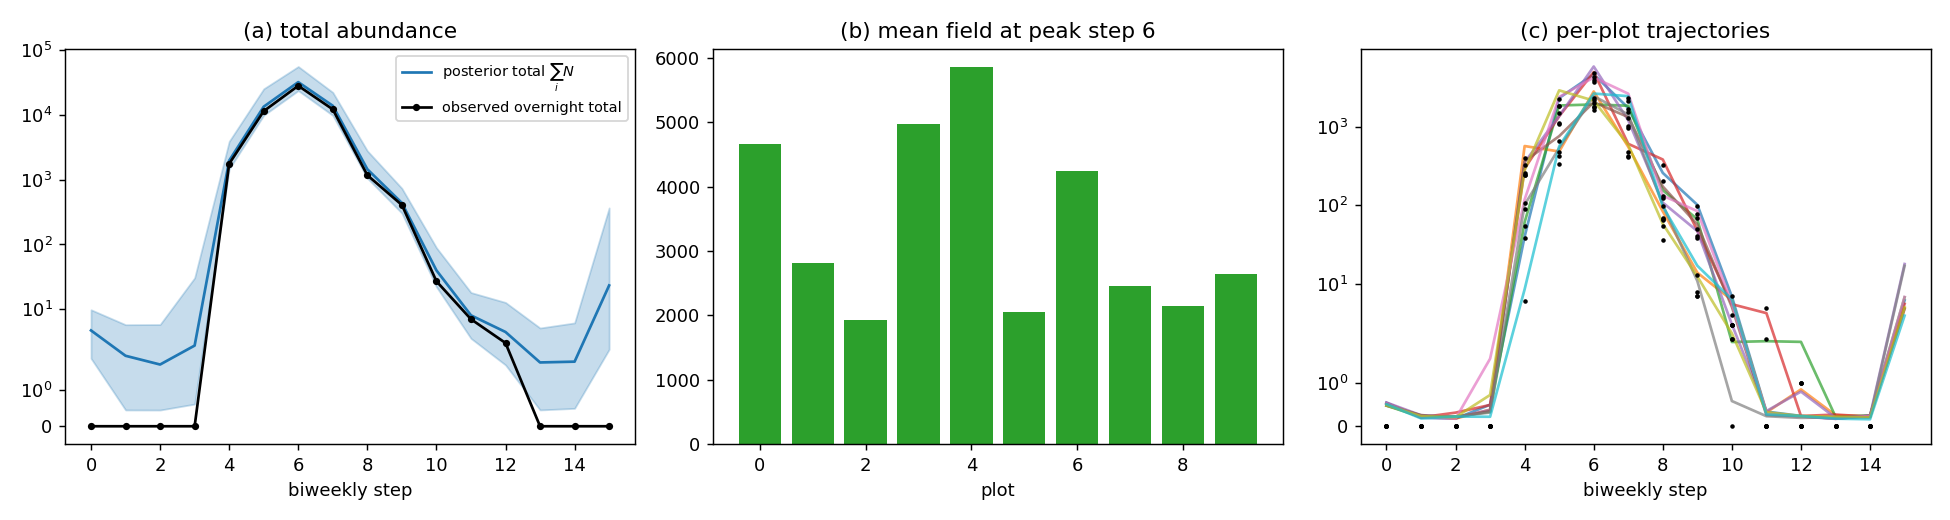
\includegraphics[width=\textwidth]{mos_field.png}
\caption{Latent abundance field for \emph{Coquillettidia perturbans} at NEON
UNDE, 2024. (a)~Posterior mean total abundance $\sum_i N_{i,t}$ (band: $95\%$)
against the observed overnight-count total, recovering a single mid-summer
boom-and-bust; (b)~posterior mean latent field $\hat N_{i,t}$ across the ten
plots at the seasonal peak, higher in the wetland-associated plots; (c)~posterior
mean per-cell trajectories (lines) with the overnight counts (points) on a
symmetric-log scale.}
\label{fig:mos-field}
\end{figure}

\begin{figure}[t]
\centering
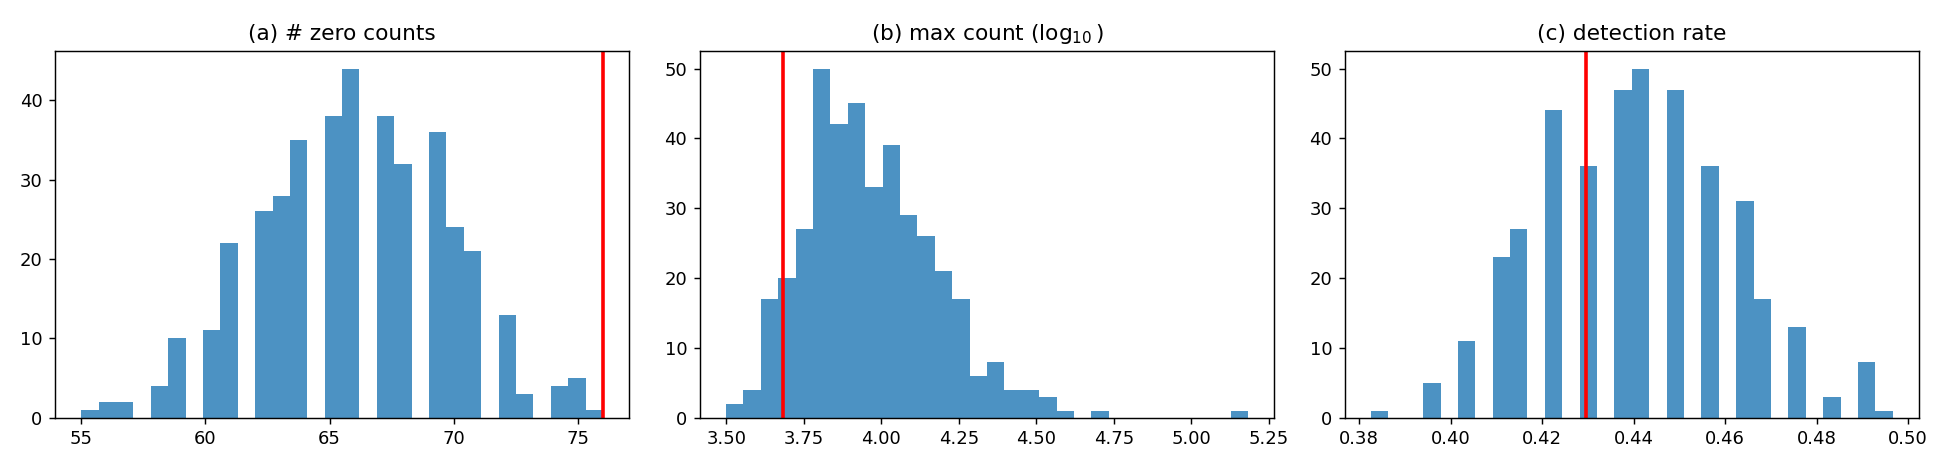
\includegraphics[width=\textwidth]{mos_ppc.png}
\caption{Posterior predictive checks for the NEON UNDE fit. Replicated
distributions (histograms) with the observed statistics (red): (a)~the number of
zero overnight counts, (b)~the maximum overnight count ($\log_{10}$ scale), and
(c)~the daytime detection rate. The observed statistics fall within their
posterior predictive distributions, indicating the dual-channel model reproduces
the zero-inflation, the heavy right tail of the counts, and the detection rate.}
\label{fig:mos-ppc}
\end{figure}

The latent field (Figure~\ref{fig:mos-field}) recovers a coherent seasonal
abundance surface---near zero in spring, a sharp mid-summer peak, and autumn
decline---with substantial spatial heterogeneity across plots, even though the
two raw streams are noisy and partly missing. Its \emph{shape} is well recovered;
its absolute level is anchored by $\rho=1$ rather than sharply pinned by the data
(the posterior for the peak total abundance is wide). The model reproduces the
key features of both channels in posterior predictive checks
(Figure~\ref{fig:mos-ppc}): the number of zero counts, the heavy right tail of
the overnight counts, and the daytime detection rate all fall within their
predictive distributions. Taken together, the application shows that the fused
count-plus-detection likelihood, fit to two genuinely independent real
observation mechanisms \emph{for the same focal species}, yields an interpretable
abundance field and observation-parameter estimates whose identifiability matches
the theory of Section~\ref{sec:ident}: the count channel carries the relative
abundance and overdispersion, and the informative species-specific binary channel
identifies both the false-positive floor and the detection intensity through the
abundance variation and the count-channel anchor.

We stress that this application demonstrates the fusion mechanism on real data,
while the \emph{quantitative} value-of-information claim---coverage and error
under a known truth---rests on the controlled simulation of
Section~\ref{sec:voi}. Two features of the fit bound what it claims. First, we
fix $\rho=1$ to anchor the abundance scale to the overnight-count channel, so the
count-detection fraction is not itself estimated here and the recovery of $\rho$
established in Proposition~\ref{prop:ident}(i) is not exercised by these data;
consequently the \emph{absolute} abundance level is only weakly identified.
Second---and this corrects an error in the previous version of this
application---the binary channel is defined \emph{species-specifically}
(detection rate $0.43$); an earlier ``any-taxon'' construction gave a
near-saturated rate ($0.77$) that made $\kappa$ appear weakly identified, but
that flag does not observe the same latent field as the count channel and has
been replaced. With the coherent species-specific channel the detection
parameters $(\kappa,\eta)$ are identified as the theory predicts; what the real
data do \emph{not} pin sharply is the absolute scale, by construction.

% ─────────────────────────────────────────────────────────────────────────────
% ─────────────────────────────────────────────────────────────────────────────
\section{Discussion}
\label{sec:discussion}
% -----------------------------------------------------------------------------

We have treated the multi-source observation model for count-valued
spatio-temporal ABMs as a subject in its own right: a stable latent process
(Theorem~\ref{thm:ergodic}, Proposition~\ref{prop:meanbound}) observed
through two conditionally independent channels whose joint identifiability we
characterised analytically (Proposition~\ref{prop:ident}) and whose practical
payoff we quantified in simulation and then in a real application: a fit to NEON
dual-channel mosquito surveillance data (Section~\ref{sec:neon-mosq}) that
recovers a coherent seasonal abundance field and observation parameters whose
relative identifiability matches the theory. The division of labour between the
two empirical sections is deliberate: the value-of-information claim---that
fusion recovers detection parameters neither stream identifies alone---rests on
the controlled simulation of Section~\ref{sec:voi}, where the truth is known and
coverage can be measured, whereas the NEON fit shows that the predicted
identifiability pattern survives real, noisy, partially missing dual-channel
data. With the corrected species-specific detection channel the informative
binary stream identifies $(\kappa,\eta)$ as the theory predicts. The one quantity
the real data do not pin sharply is the \emph{absolute} abundance scale: we fix
$\rho=1$ to anchor the scale to the count channel, so the count-detection
fraction is not estimated there, and with many zero and low-count cells the
level of the latent field is set by the anchor and priors rather than by the data
(the peak-abundance posterior is wide). We are careful not to over-read the
application on this point: it demonstrates the fusion mechanism and the
identifiability of the detection parameters, but not a data-driven absolute
abundance.

\paragraph{Implications for monitoring design.}
The results speak directly to survey design. First, a second stream is
worth collecting precisely when the count channel leaves detection and
abundance confounded and no strong prior or replication pins the scale: the
value-of-information experiment shows count-only data cannot estimate the
binary detection rate at all, and binary-only data forecast abundance
poorly, while fusion recovers both. Second, temporal replication is
essential for the binary channel: a single presence/absence occasion cannot
separate true detection from false positives
(Proposition~\ref{prop:ident}(ii), Remark~\ref{rmk:necessary}), so
occupancy-style repeat visits or a multi-year design are prerequisites, not
refinements. Third, habitat remote-sensing products should not be entered as
detections without a false-positive model; in the mosquito application,
land-cover covariates enter the latent process, whereas trap effort enters the
observation layer.

\paragraph{Limitations.}
The identifiability results are conditional on positive latent counts and
are local (Fisher-information) statements; converting them to global,
fully hierarchical identifiability requires process-dependent conditions we
do not establish here (Remark~\ref{rmk:conditional}). Near the unit-root
regime the long-distance arrival rate is weakly separated from the count
detection fraction, which is why the mosquito fit anchors the abundance scale
through the count channel ($\rho{=}1$) rather than estimating the
count-detection fraction and the arrival rate jointly---so the \emph{absolute}
abundance scale in the application is set by the anchor rather than the data. An
alternative to fixing $\rho=1$ is to free $\rho$ under an informative
$\mathrm{N}(\mu_\rho^0,\sigma_0^2)$ prior, which would report an absolute scale
\emph{with} honest posterior uncertainty and exercise
Proposition~\ref{prop:ident}(i) on the real data; our released fitting code
(\texttt{mos\_numpyro\_fit.py}) exposes this option. The
false-positive rate $\eta$ is only weakly identified from a short binary series
and benefits from an informative prior; our sensitivity analysis suggests
estimates are robust to small $\eta$, but datasets with substantial false
positives would need a richer proxy model. A further lesson from the application
is that the two channels must observe the \emph{same} latent quantity: a coarse
``any-taxon'' detection flag is near-saturated and does not identify the focal
species' detection parameters, whereas the species-specific channel used here
does. Finally, the real application is a single site and season with $m=10$
plots; extending the same dual-channel likelihood to larger, multi-programme
integrations---for example BBS route counts fused with eBird detections over
continental grids---is a natural next step.

\paragraph{Scope of the present article.}
The manuscript deliberately avoids claims about flexible kernel learning or
computational acceleration. Those topics can be studied with many different
implementations, but they are secondary to the central statistical issue
addressed here: whether the fused observation likelihood separates abundance,
count detection, binary detection intensity, and false positives. This focus
makes the paper independent and suitable as a statistical-ecology contribution
to integrated monitoring design.

% -----------------------------------------------------------------------------
% -----------------------------------------------------------------------------
\appendix
\section{Supporting simulation studies}
\label{app:supporting}
% -----------------------------------------------------------------------------

Two further self-contained studies, released with the paper, support the claims
of Sections~\ref{sec:voi} and~\ref{sec:neon-mosq}. Both isolate a single
question and neither depends on the choice of dispersal kernel or fitting
algorithm, consistent with the paper's scope.

\paragraph{The count-only abundance scale is data-driven, not prior-driven.}
Section~\ref{sec:voi} reports that count-only data (regime~R1) recover the
detection intercept $\mu_\rho$. Table~\ref{tab:app-scale} confirms that this
recovery is supplied by the density-dependent dynamics rather than by the prior.
Jointly estimating $(\mu_\rho,K)$---and hence the absolute abundance scale---from
a single count-only series by an exact truncated forward filter, the posterior
mean of $\mu_\rho$ stays near the truth ($-0.5$) and the implied mean abundance
$\hat N$ is essentially invariant ($\approx\!10.7$, true value $\approx\!10.6$)
as the $\mu_\rho$ prior is moved from $\mathcal N(0,0.5^2)$ to $\mathcal
N(-1.5,1)$: a five-fold change in prior location shifts $\hat N$ by under
$1\%$. The density-regulated approach to carrying capacity gives the count
series a shape that pins the level, so $\mu_\rho$ is identified by the data.

\begin{table}[t]
\centering\small\renewcommand{\arraystretch}{1.2}
\begin{tabular}{lccc}
\toprule
$\mu_\rho$ prior & post.\ mean $\mu_\rho$ & $\bar\rho$ & $\hat N$ \\
\midrule
$\mathcal N(0,0.5^2)$ (tight) & $-0.30$ & $0.426$ & $10.67$ \\
$\mathcal N(0,1)$ (main)      & $-0.39$ & $0.406$ & $10.72$ \\
$\mathcal N(0.5,1)$           & $-0.33$ & $0.420$ & $10.69$ \\
$\mathcal N(-1.5,1)$          & $-0.55$ & $0.369$ & $10.79$ \\
\bottomrule
\end{tabular}
\caption{Count-only joint estimation of $(\mu_\rho,K)$ under varying $\mu_\rho$
priors (truth $\mu_\rho=-0.5$, mean $N\approx10.6$; carrying-capacity prior
anchored; exact truncated forward filter). The implied abundance scale $\hat N$
is nearly invariant to the prior, so the scale is data-driven
(\texttt{joint\_estimation\_study.py}).}
\label{tab:app-scale}
\end{table}

\paragraph{Low-count behaviour of the transition surrogate.}
Table~\ref{tab:app-lowcount} quantifies the caveat of Section~\ref{sec:neon-model}
by comparing bootstrap particle filters that differ only in their one-step
transition---the exact Binomial--Poisson law, its moment-matched Gaussian
surrogate, and the log-normal surrogate used in the NEON fit---against the true
latent field. In the application abundance regime (mean count $\approx\!9.5$,
the summer plot-years) all three agree closely, with $90\%$ credible-interval
coverage $0.90$--$0.93$. In the low-count regime (mean count $\approx\!1.2$, the
spring and zero-inflated plot-years) the Gaussian surrogate is indistinguishable
from the exact filter, whereas the log-normal surrogate degrades: its coverage
falls to $0.64$ and, unlike the exact and Gaussian laws, it cannot place mass at
$N=0$ (at $\mu=1.5$ the exact transition has $\Pr(N=0)=0.12$ against $0.04$ for
the log-normal). This locates the numerical error flagged in
Section~\ref{sec:neon-model} precisely at the near-zero counts. The comparison is
made in stationary regimes; for the strongly non-stationary mosquito series we
retain the log-normal surrogate for the boom-bust reasons given in
Section~\ref{sec:neon-model}, and note that an exact truncated-filter or particle
treatment is the assumption-free route to eliminating the residual low-count
error.

\begin{table}[t]
\centering\small\renewcommand{\arraystretch}{1.2}
\begin{tabular}{llcc}
\toprule
Regime (mean $N$) & Transition & latent-field RMSE & $90\%$ cov. \\
\midrule
\multirow{3}{*}{Low ($\approx1.2$)}
 & exact       & $0.879$ & $0.970$ \\
 & Gaussian    & $0.877$ & $0.971$ \\
 & log-normal  & $0.912$ & $0.637$ \\
\midrule
\multirow{3}{*}{Application ($\approx9.5$)}
 & exact       & $2.610$ & $0.930$ \\
 & Gaussian    & $2.601$ & $0.934$ \\
 & log-normal  & $2.606$ & $0.900$ \\
\bottomrule
\end{tabular}
\caption{Latent-field recovery of particle filters differing only in the
one-step transition law, against the true field. The Gaussian surrogate matches
the exact filter in both regimes; the log-normal surrogate undercovers in the
low-count regime, where it cannot represent $\Pr(N=0)$
(\texttt{low\_count\_study.py}).}
\label{tab:app-lowcount}
\end{table}

% -----------------------------------------------------------------------------
\section*{Data and Code Availability}
% -----------------------------------------------------------------------------

The NEON mosquito surveillance data (overnight $\mathrm{CO}_2$-trap counts and
daytime-trap detections) analysed in Section~\ref{sec:neon-mosq} are openly
available from the National Ecological Observatory Network data portal
\citep{neon2024}. The North American Breeding Bird Survey and eBird Basic Dataset
referenced as a natural extension are available, respectively, from the USGS BBS
data release \citep{usgsbbs2022} and from eBird after a data request
\citep{ebirddata2026}. The full analysis code is released as a versioned repository archived at a
public DOI (Zenodo, \url{https://doi.org/10.5281/zenodo.XXXXXXX}; mirrored on OSF at
\url{https://osf.io/XXXXX}), snapshotted at the git tag used for this article and
accompanied by an environment specification for exact reproduction. The
repository contains the reference model implementation
(\texttt{sc\_abm\_model.py}); the value-of-information simulation and estimator
of Section~\ref{sec:voi-methods}; the process-validation experiments of
Section~\ref{sec:sim-validation}; and the supporting studies of
Appendix~\ref{app:supporting} (\texttt{joint\_estimation\_study.py},
\texttt{low\_count\_study.py}) together with the transition-approximation
characterisation of Section~\ref{sec:neon-model}
(\texttt{approx\_error\_study.py}). All scripts use fixed pseudo-random seeds so
that every figure and table is reproducible from a clean checkout.

\subsection{Robustness of the value-of-information analysis}
\label{app:robust}

The coverage figures of Section~\ref{sec:voi} are produced with the demographic
process held at its data-generating values and at a moderate abundance. Three
further checks (released as \texttt{paper2\_sim\_studies.py}; $R=20$ replicates,
$m=35$, $T=18$; exact forward-filter marginal likelihood, Laplace $95\%$
intervals) probe how far those figures survive the conditions of the real
application. Table~\ref{tab:robust} reports the results.

\begin{table}[h!]
\centering\small\renewcommand{\arraystretch}{1.2}
\begin{tabular}{llcc}
\toprule
\textbf{Check} & \textbf{Setting} & $\mu_\rho$ cov.\ (width) & $\kappa$ cov.\ (width)\\
\midrule
\multirow{2}{*}{Process nuisance}
 & $(\phi,\psi,K)$ fixed at truth & $1.00\ (0.22)$ & $0.95\ (0.020)$\\
 & $(\phi,\psi,K)$ estimated jointly & $0.95\ (1.49)$ & $0.95\ (0.129)$\\
\midrule
\multirow{2}{*}{Abundance regime}
 & moderate ($\bar N\!\approx\!7.5$, $24\%$ zeros) & $0.90\ (0.23)$ & $1.00\ (0.020)$\\
 & low ($\bar N\!\approx\!1.5$, $72\%$ zeros)      & $0.95\ (0.43)$ & $0.95\ (0.080)$\\
\bottomrule
\end{tabular}
\caption{Coverage of nominal $95\%$ intervals ($R=20$; Monte Carlo standard
error $\le0.11$). Coverage is maintained when the process is estimated jointly
and in the low-abundance/high-zero regime, but the intervals widen sharply
(the $\kappa$ interval is $\sim\!6\times$ wider with the process estimated, and
$\sim\!4\times$ wider at low abundance): the fixed-process, moderate-abundance
figures of Section~\ref{sec:voi} are therefore optimistic about \emph{precision},
though not about \emph{calibration}.}
\label{tab:robust}
\end{table}

A third check varies the false-positive prior (true $\eta^\star=0.15$). With a
correctly informative prior ($\mathrm{Beta}(3,17)$) both $\eta$ and $\kappa$ are
recovered with near-nominal coverage; under a \emph{diffuse} prior
($\mathrm{Beta}(1,1)$) the $\eta$ coverage falls to $0.80$ and the joint
$(\kappa,\eta)$ estimate becomes unstable; under a \emph{mis-centred} prior
($\mathrm{Beta}(1,49)$, mean $0.02$) the resulting $\eta$ bias propagates to
$\kappa$, whose coverage collapses to $0.00$. The false-positive rate is thus
only weakly identified from a short binary series and is materially
prior-dependent---an informative, correctly-centred prior is a modelling
requirement, not a convenience, and a mis-specified one is actively harmful. This
sharpens the limitation already noted in Section~\ref{sec:discussion}.

% -----------------------------------------------------------------------------
\section*{Acknowledgements}
% -----------------------------------------------------------------------------

We thank the volunteers and coordinators of the North American Breeding Bird
Survey and the eBird community for making large-scale bird-monitoring data
available for scientific use. We are grateful to Professor Dennis K.\ J.\ Lin
(Purdue University) for helpful discussions. This work was supported by the
National Natural Science Foundation of China (grant no.\ 11461079).

% -----------------------------------------------------------------------------

\begin{thebibliography}{99}

\bibitem[Kery and Royle(2016)]{kery2016}
Kery, M., and Royle, J. A. (2016).
\newblock \emph{Applied Hierarchical Modeling in Ecology: Analysis of Distribution, Abundance and Species Richness in R and BUGS}.
\newblock Academic Press.

\bibitem[Royle(2004)]{royle2004}
Royle, J. A. (2004).
\newblock N-mixture models for estimating population size from spatially replicated counts.
\newblock \emph{Biometrics}, 60(1), 108--115.

\bibitem[Dail and Madsen(2011)]{dail2011}
Dail, D., and Madsen, L. (2011).
\newblock Models for estimating abundance from repeated counts of an open metapopulation.
\newblock \emph{Biometrics}, 67(2), 577--587.

\bibitem[Link(2003)]{link2003}
Link, W. A. (2003).
\newblock Nonidentifiability of population size from capture--recapture data with heterogeneous detection probabilities.
\newblock \emph{Biometrics}, 59(4), 1123--1130.

\bibitem[Knape and Korner-Nievergelt(2015)]{knape2015}
Knape, J., and Korner-Nievergelt, F. (2015).
\newblock Estimates from non-replicated population surveys rely on critical assumptions.
\newblock \emph{Methods in Ecology and Evolution}, 6(3), 298--306.

\bibitem[Barker et~al.(2018)]{barker2018}
Barker, R. J., Schofield, M. R., Link, W. A., and Sauer, J. R. (2018).
\newblock On the reliability of N-mixture models for count data.
\newblock \emph{Biometrics}, 74(1), 369--377.

\bibitem[Meyn and Tweedie(2009)]{meyntweedie2009}
Meyn, S. P., and Tweedie, R. L. (2009).
\newblock \emph{Markov Chains and Stochastic Stability}.
\newblock Cambridge University Press.

\bibitem[Gneiting and Raftery(2007)]{gneiting2007}
Gneiting, T., and Raftery, A. E. (2007).
\newblock Strictly proper scoring rules, prediction, and estimation.
\newblock \emph{Journal of the American Statistical Association}, 102(477), 359--378.

\bibitem[Hooten and Wikle(2010)]{hooten2010}
Hooten, M. B., and Wikle, C. K. (2010).
\newblock Statistical agent-based models for discrete spatio-temporal systems.
\newblock \emph{Journal of the American Statistical Association}, 105(489), 236--248.

\bibitem[Nathan et~al.(2012)]{nathan2012}
Nathan, R., Klein, E., Robledo-Arnuncio, J. J., and Revilla, E. (2012).
\newblock Dispersal kernels: review.
\newblock In J. Clobert, M. Baguette, T. G. Benton, and J. M. Bullock (eds.), \emph{Dispersal Ecology and Evolution}, pp. 187--210. Oxford University Press, Oxford.

\bibitem[Isaac et~al.(2020)]{isaac2020}
Isaac, N. J. B., Jarzyna, M. A., Keil, P., Dambly, L. I., Boersch-Supan, P. H., Browning, E., Freeman, S. N., Golding, N., Guillera-Arroita, G., Henrys, P. A., Jarvis, S., Lahoz-Monfort, J. J., Pagel, J., Pescott, O. L., Schmucki, R., Simmonds, E. G., and O'Hara, R. B. (2020).
\newblock Data integration for large-scale models of species distributions.
\newblock \emph{Trends in Ecology \& Evolution}, 35(1), 56--67.

\bibitem[Doser et~al.(2023)]{doser2023}
Doser, J. W., Finley, A. O., and Banerjee, S. (2023).
\newblock Joint species distribution models with imperfect detection for high-dimensional spatial data.
\newblock \emph{Ecology}, 104(9), e4137.

\bibitem[Doser and Stoudt(2024)]{doser2024}
Doser, J. W., and Stoudt, S. (2024).
\newblock ``Fractional replication'' in single-visit multi-season occupancy models: impacts of spatiotemporal autocorrelation on identifiability.
\newblock \emph{Methods in Ecology and Evolution}, 15(2), 358--372.

\bibitem[Ver Hoef et~al.(2025)]{verhoef2025}
Ver Hoef, J. M., McClintock, B. T., Boveng, P. L., London, J. M., and Jansen, J. K. (2025).
\newblock An integrated data model to estimate abundance from counts with temporal dependence and imperfect detection.
\newblock \emph{Ecology}, 106(5), e70073.

\bibitem[Schmid et~al.(2004)]{schmid2004}
Schmid, H., Zbinden, N., and Keller, V. (2004).
\newblock Monitoring der h\"aufigen Brutv\"ogel (MHB): Monitoring the common breeding birds in Switzerland.
\newblock Swiss Ornithological Institute, Sempach.

\bibitem[NEON(2024)]{neon2024}
National Ecological Observatory Network (NEON) (2024).
\newblock Mosquitoes sampled from CO2 traps (DP1.10043.001), RELEASE-2024.
\newblock National Ecological Observatory Network, Boulder, Colorado, USA. Available from \url{https://data.neonscience.org}.

\bibitem[Ziolkowski et~al.(2022)]{usgsbbs2022}
Ziolkowski, D. J., Lutmerding, M., Aponte, V. I., and Hudson, M.-A. R. (2022).
\newblock 2022 release: North American Breeding Bird Survey Dataset (1966--2021).
\newblock U.S. Geological Survey data release, doi:10.5066/P97WAZE5.

\bibitem[Cornell Lab of Ornithology(2024)]{ebirddata2026}
Cornell Lab of Ornithology (2024).
\newblock eBird Basic Dataset (EBD).
\newblock Cornell Lab of Ornithology, Ithaca, New York. Available from \url{https://ebird.org/data/download}.

\end{thebibliography}

\end{document}
